\subsection{Heap} % (fold)
\label{sub:heap}

When your program is executed it allocated memory to work with.

\begin{figure}[h]
   \centering
   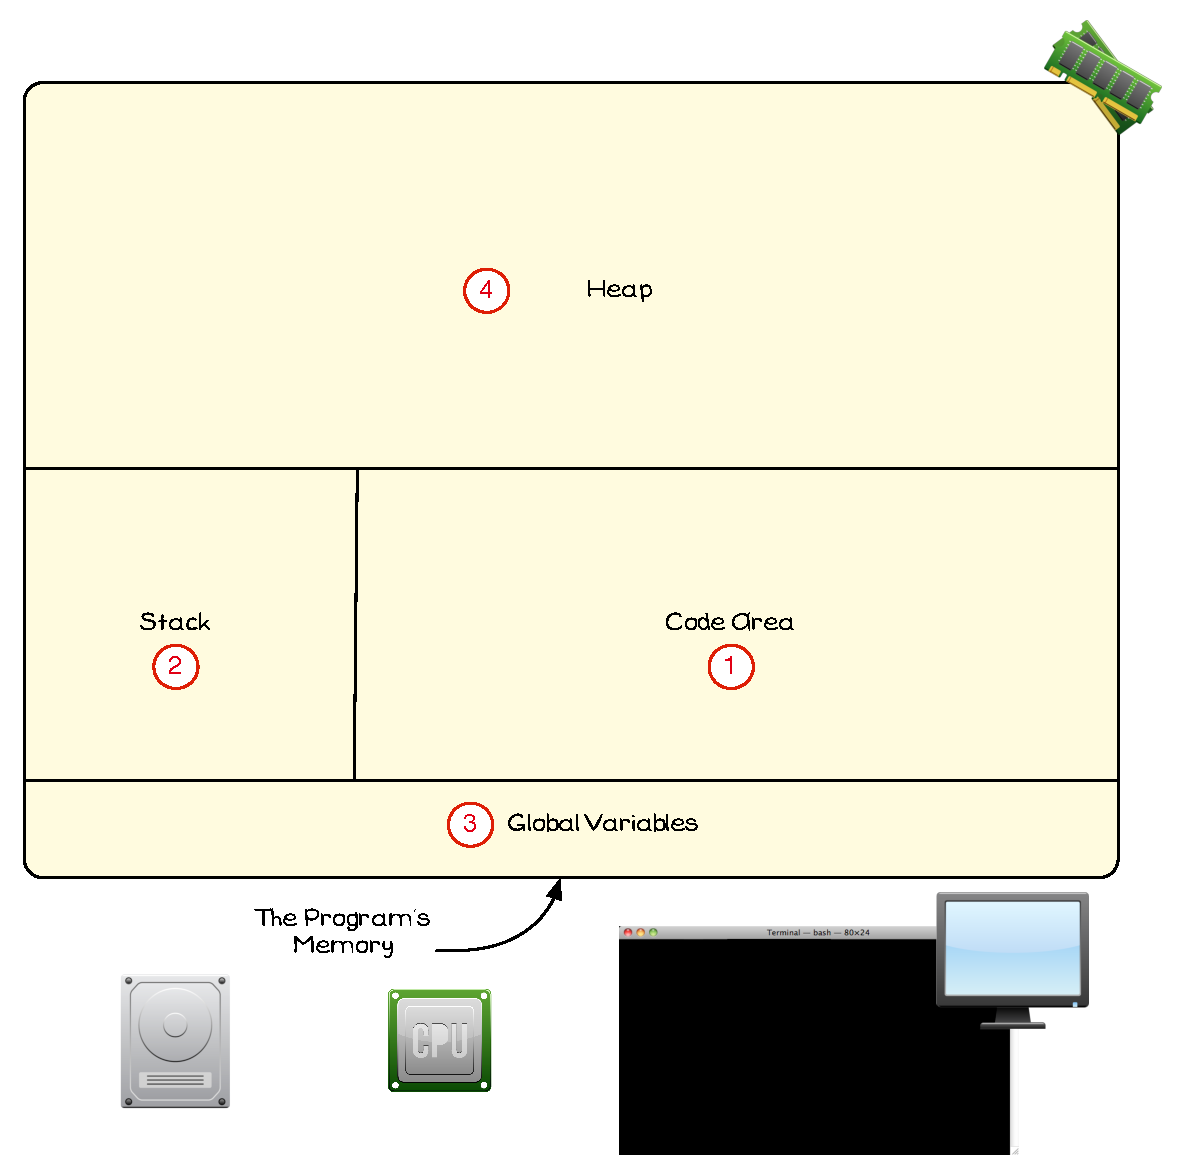
\includegraphics[width=0.8\textwidth]{./topics/dynamic-memory/diagrams/Heap} 
   \caption{Arrays allow you to store multiple values in a variable}
   \label{fig:heap}
\end{figure}

\mynote{
\begin{itemize}
  \item \fref{fig:heap} includes the following areas:
  \begin{enumerate}
    \item Your program's machine code is loaded into the \textbf{Code Area}.
    \item The \textbf{Stack} is used to manage the execution of the program's functions and procedures.
    \item \textbf{Global Variables} are allocated their own space.
    \item The new area is the \textbf{Heap}. This is used to store all dynamically allocated values.
  \end{enumerate}
  \item Values can be stored in the \emph{global variables}, in local variables on the \emph{Stack}, and on the \emph{Heap} using dynamic memory allocation functions and procedures.
  \item The space taken up by the \textbf{global variables} is fixed based on the size of the variables you have declared.
  \item Each function/procedure takes a fixed amount of space on the stack. The space allocated is enough to store each of the local variables, plus some additional space for various overheads.
\end{itemize}
}


% subsection heap (end)